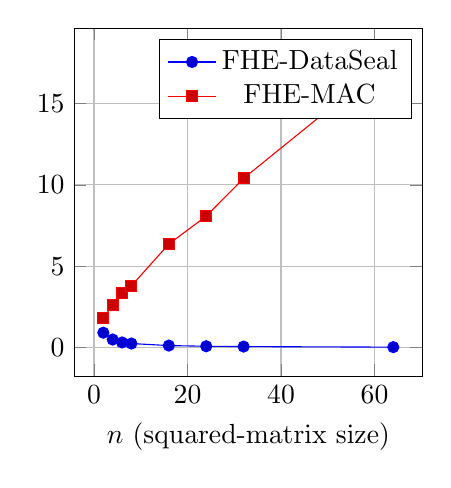
\begin{tikzpicture}
\begin{axis}[
    width=6cm, % Set the width of the plot to the text width of the subfigure
    height=6cm, % You can adjust the height as needed
    xlabel={$n$ (squared-matrix size)},
    % ylabel={Time in Seconds},
    legend pos=north east,
    grid=both,
    % xmin=1, xmax=64,
    % ymin=0, ymax=80
]

% \addplot table {
% n	FHE-TEE
% 2	0.108531995
% 4	0.1112679893
% 6	0.1201377863
% 8	0.1202104645
% 16	0.125836684
% 24	0.1297872057
% 32	0.1297466707
% 64  0.1325926569
% };
% \addlegendentry{FHE-TEE}

\addplot table {
n	vFHE
% 1   0.9552
2	0.9168
4	0.4978
6	0.3183
8	0.2507
16	0.1258
24	0.0839
32	0.0634
64  0.030124852
};
\addlegendentry{FHE-DataSeal}

\addplot table {
n   FHE+MAC
2	1.808455935
4	2.625042594
6	3.367575084
8	3.798410581
16	6.363348129
24	8.082796059
32	10.40652348
64	17.85042956
};
\addlegendentry{FHE-MAC}

\end{axis}
\end{tikzpicture}